\documentclass[preview,border=6pt,varwidth=84mm,11pt]{standalone}
\usepackage[T1]{fontenc}
\usepackage[utf8]{inputenc}
\usepackage{amsmath,amssymb}
\usepackage{tikz}
\usetikzlibrary{automata,positioning,arrows.meta}
\usepackage{graphicx}
\usepackage{booktabs}
\usepackage{enumitem}
\setlength{\parindent}{0pt}
\begin{document}
Nacrtati automat sa dva stanja: početno $q_0$ i završno $q_1$ (čćšžđ ČĆŠŽĐ).

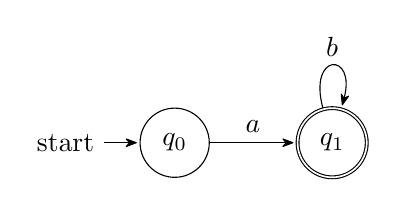
\begin{tikzpicture}[shorten >=1pt, node distance=2cm, on grid, auto, >={Stealth[round]}]
  \node[state, initial] (q0) {$q_0$};
  \node[state, accepting, right=of q0] (q1) {$q_1$};
  \path[->] (q0) edge node {$a$} (q1)
            (q1) edge[loop above] node {$b$} ();
\end{tikzpicture}

\begin{enumerate}[label=\alph*)]
  \item $\sum_{i=1}^{n} i = \frac{n(n+1)}{2}$
  \item $x \in \mathbb{N}$
\end{enumerate}

\begin{tabular}{@{}lr@{}}
  \toprule
  Stanje & Izlaz \\
  \midrule
  $q_0$ & 0 \\
  $q_1$ & 1 \\
  \bottomrule
\end{tabular}

\includegraphics[width=1cm]{slika}
\end{document}
